\section{\numb section 3. Progressive mesh generation}

Section \numb section 2 shows how to build meshes by joining rectangles and triangles together,
like patches.
The present section explains how to build a mesh starting from its boundary only;
we call this approach ``progressive mesh generation''.
It consists of starting with a given interface and add triangles, one by one,
moving and deforming the interface, until it shrinks and disappears.
In some cases (like in paragraphs \numb section 3.\numb parag 2, \numb section 3.\numb parag 4,
\numb section 3.\numb parag 6, \numb section 3.\numb parag 7) we begin with nothing at all;
{\maniFEM} finds a starting point by itself.

Progressive mesh generation works with segment cells (for one-dimensional meshes) and
triangular cells (for two-dimensional meshes).
Meshing of three-dimensional domains will be implemented in the future and will use tetrahedral
cells.

Progressive mesh generation follows the shape of the current working manifold (the most recently
declared {\codett Manifold} object) by {\codett project}ing each newly constructed vertex
on that manifold.
Recall that in this manual we use the term ``manifold'' to mean a manifold without boundary.


\paragraph{\numb section 3.\numb parag 1. Filling a disk}

Paragraph \numb section 2.\numb parag 8 shows how to build a mesh over a disk,
but the quality of the mesh is quite poor.
This is so because the {\codett Mesh} constructor with {\codett tag::quadrangle} treats the
disk as a (much) deformed rectangle.

We can ask {\maniFEM} to progressively mesh the disk, starting from its boundary (a circle)
and adding triangles, one by one, until the disk is completely covered :

\centerline{\includegraphics[width=75mm]{disk-with-tri.eps}}

\verbatim
   Manifold RR2 ( tag::Euclid, tag::of_dim, 2 );
   Function xy = RR2.build_coordinate_system ( tag::Lagrange, tag::of_degree, 1 );
   Function x = xy[0],  y = xy[1];
   
   Manifold circle_manif = RR2.implicit ( x*x + y*y == 1. );
   
   Cell N ( tag::vertex );  x(N) =  0.;   y(N) =  1.;
   Cell W ( tag::vertex );  x(W) = -1.;   y(W) =  0.;
   Cell S ( tag::vertex );  x(S) =  0.;   y(S) = -1.;
   Cell E ( tag::vertex );  x(E) =  1.;   y(E) =  0.;
   Mesh NW ( tag::segment, N.reverse(), W, tag::divided_in, 10 );
   Mesh WS ( tag::segment, W.reverse(), S, tag::divided_in, 10 );
   Mesh SE ( tag::segment, S.reverse(), E, tag::divided_in, 10 );
   Mesh EN ( tag::segment, E.reverse(), N, tag::divided_in, 10 );
   Mesh circle ( tag::join, NW, WS, SE, EN );
   
   RR2.set_as_working_manifold();
   Mesh disk ( tag::progressive, tag::boundary, circle, tag::desired_length, 0.157 );
\endverbatim

We provide the desired length of the segments of the future mesh as an argument to the
constructor.
Of course the length of the segments inside the mesh will vary slightly.
We must take care to give as boundary a curve with segments of length approximatively equal
to the desired length (paragraph \numb section 3.\numb parag 16 discusses this requirement).

Paragraph \numb section 10.\numb parag 2 gives more details about {\codett tag}s.


\paragraph{\numb section 3.\numb parag 2. Meshing a circle}

Instead of building the circle by joining four (curved) segments, we can mesh directly
the circle manifold, then mesh the disk :

\verbatim
   Manifold RR2 ( tag::Euclid, tag::of_dim, 2 );
   Function xy = RR2.build_coordinate_system ( tag::Lagrange, tag::of_degree, 1 );
   Function x = xy[0],  y = xy[1];
   
   Manifold circle_manif = RR2.implicit ( x*x + y*y == 1. );
   Mesh circle ( tag::progressive,
      tag::entire_manifold, circle_manif, tag::desired_length, 0.2 );
   // we can omit the manifold; maniFEM will take the current working manifold :
   // Mesh circle ( tag::progressive, tag::desired_length, 0.2 );
   
   RR2.set_as_working_manifold();
   Mesh disk ( tag::progressive, tag::boundary, circle, tag::desired_length, 0.2 );
   disk.draw_ps ("disk.eps");
\endverbatim

The code above is quite comfortable for the user; he or she only needs to define
the manifold(s) to be meshed and provide the desired (average) length of segments
in the future mesh.
However, this comfort comes at the price of a significant computational effort.
For building the {\codett circle}, {\ManiFEM} must first find a starting point for the process
of progressive mesh generation.
In extreme cases, the algorithm may fail to find a starting point on the given manifold.

The user may choose to be more specific in order to save computation time,
by providing a starting point :

\verbatim
   Cell A ( tag::vertex );  x(A) = 1.;  y(A) = 0.;
   Mesh circle ( tag::progressive, tag::start_at, A, tag::desired_length, 0.2 );
\endverbatim

Also, {\maniFEM} must infer the right orientation of the {\codett circle}
as explained in paragraphs \numb section 3.\numb parag 10 and \numb section 3.\numb parag 13.
Choosing the other orientation would result in an endless process of meshing the exterior of
the disk.
The process of choosing the right orientation implies some computational effort.
The user can make things easier for {\maniFEM} either by attaching an orientation
to the manifold {\codett circle\_manif} (this feature is not implemented yet)
or by providing the initial direction as shown in paragraph \numb section 3.\numb parag 12.


\paragraph{\numb section 3.\numb parag 3. Inner boundaries}

Inner boundaries must have the reverse orientation :

\verbatim
   Manifold circle = RR2.implicit ( x*x + y*y == 1. );
   Mesh outer ( tag::progressive, tag::desired_length, 0.1 );
   Manifold ellipse = RR2.implicit ( x*x + (y-0.37)*(y-0.37) + 0.3*x*y == 0.25 );
   Mesh inner ( tag::progressive, tag::desired_length, 0.1 );
   Mesh bdry ( tag::join, outer, inner.reverse() );
   RR2.set_as_working_manifold();
   Mesh disk ( tag::progressive, tag::boundary, bdry, tag::desired_length, 0.1 );
   \endverbatim

\centerline{\includegraphics[width=90mm]{disk-with-hole.eps}}

Paragraph \numb section 1.\numb parag 2 explains the relation between the orientation of
a mesh and the orientation of its boundary.

Paragraphs \numb section 3.\numb parag 10 and \numb section 3.\numb parag 13 explain how
{\maniFEM} chooses the orientation of closed curves.


\vskip 5mm
\paragraph{\numb section 3.\numb parag 4. Meshing a three-dimensional loop}

We may apply the same {\codett progressive} algorithm for meshing the circle in $ \RR^3 $
introduced in paragraph \numb section 2.\numb parag 11 :

\verbatim
   Manifold RR3 ( tag::Euclid, tag::of_dim, 3 );
   Function xyz = RR3.build_coordinate_system ( tag::Lagrange, tag::of_degree, 1 );
   Function x = xyz[0],  y = xyz[1],  z = xyz[2];

   Manifold circle_manif = RR3.implicit ( x*x + y*y == 1., x*y == 4.*z );
   
   Mesh circle
      ( tag::progressive, tag::desired_length, 0.1, tag::random_orientation );
\endverbatim

Unlike for the {\codett circle} in paragraph \numb section 3.\numb parag 2, there is no way
to choose between the two possible orientations of this {\codett circle}.
No one is more ``correct'' than the other.
This is why {\maniFEM} requires a supplementary argument {\codett tag::random\_orientation}
for the {\codett Mesh} constructor.
This supplementary argument can be used even when it is not mandatory (like in the case of
closed curves in $ \RR^2 $), thus sparing the computer from the burden of finding
the right orientation.
Paragraphs \numb section 3.\numb parag 10 and \numb section 3.\numb parag 13 give more details.

On the other hand, if the orientation matters for you, you can either attach an orientation
to the manifold {\codett circle\_manif} (this feature is not implemented yet)
or provide a starting point and an initial direction as shown in paragraph
\numb section 3.\numb parag 12.


\paragraph{\numb section 3.\numb parag 5. Starting and stopping points}

In paragraphs \numb section 3.\numb parag 2 andd \numb section 3.\numb parag 4 we have meshed
the entire closed curve {\codett circle}.
If we only want a piece of a curve, we must specify two points, one for starting and
the other one for stopping.

Looking at the example in paragraph \numb section 2.\numb parag 13, let us define a
spiral with a slightly different look and switch to progressive mesh generation.

{ \psfrag{A}{\special{ps: gsave 0 0 0.8 setrgbcolor}{\codett A}\special{ps: grestore}}
\psfrag{B}{\special{ps: gsave 0 0 0.8 setrgbcolor}{\codett B}\special{ps: grestore}}
\centerline{\includegraphics[width=75mm]{spiral-prog.eps}}}

\verbatim
   Manifold RR2 ( tag::Euclid, tag::of_dim, 2 );
   Function xy = RR2.build_coordinate_system ( tag::Lagrange, tag::of_degree, 1 );
   Function x = xy[0],  y = xy[1];
   Function r = power ( x*x + y*y, 0.25 );
   const double pi = 3.14159;
   
   RR2.implicit ( x*sin(r) == y*cos(r) );
   // we don't need to give a name to the implicit manifold
   // the Manifold constructor sets the manifold it builds as working manifold
   // after that, many methods use this working manifold by default
   
   Cell A ( tag::vertex );  x(A) =    pi*pi;   y(A) =  0.;
   Cell B ( tag::vertex );  x(B) = 81*pi*pi;   y(B) =  0.;
   Mesh spiral ( tag::progressive, tag::start_at, A,
                 tag::stop_at, B, tag::desired_length, 1. );
\endverbatim

Unlike in paragraph \numb section 2.\numb parag 13, we define the spiral through an implicit
equation.
Had we chosen the (natural) definition {\codett r = power ( x*x + y*y, 0.5 )},
the very same spiral as in paragraph \numb section 2.\numb parag 13 would have been obtained.
For aesthetic reasons, we have chosen a different definition of {\codett r}, thus obtaining
a different spacing between the arcs of the spiral.

Another noteworthy difference from paragraph \numb section 2.\numb parag 13 is that vertices
are distributed along the spiral uniformly (with respect to the distance in the surrounding
space $ \RR^2 $).
The segments are too small to be seen in the figure.

Note that there are two ways to go along the spiral starting from {\codett A}.
One of them will eventually stumble upon the stopping point {\codett B} while
the other one will never meet {\codett B}.
{\ManiFEM} has no means to guess which way it should start building the mesh,
so it performs a preliminary search in both directions.
The one that first meets {\codett B} wins and the mesh is subsequently built along
the winning direction.

Thus, if we want to mesh an arc of a circle, we can use a sequence of statements like

\verbatim
   RR2.implicit ( (x-x0)*(x-x0) + (y-y0)*(y-y0) == radius * radius );
   Cell A ( tag::vertex );  // set x(A) and y(A)
   Cell B ( tag::vertex );  // set x(B) and y(B)
   Mesh arc_of_circle ( tag::progressive, tag::start_at, A,
                        tag::stop_at, B, tag::desired_length, some_value );
\endverbatim

However, if we choose {\codett A} and {\codett B} diametrally opposed, {\maniFEM} will
mesh unpredictably one half of the circle or the other.

Paragraph \numb section 3.\numb parag 12 shows how we can specify the direction we
want to follow starting from a given point, thus avoiding ambiguities and also saving
computational time.

Of course we must be careful to choose starting and stopping points belonging to the manifold
(or to {\codett project} them explicitly -- for this we should have given a name to the
implicit manifold) otherwise the meshing algorithm will either fail to start or will spin
for ever on the circle or spiral, hopelessly searching for {\codett B}.


\paragraph{\numb section 3.\numb parag 6. Meshing a compact surface}

Recall that in this manual we use the term ``manifold'' to mean a manifold without boundary.
So, the term ``compact surface'' should be understood as ``compact surface without boundary''
like the sphere or the torus.

Just like for the {\codett circle} in paragraphs \numb section 3.\numb parag 2 and
\numb section 3.\numb parag 4,
if we want to mesh a compact surface entirely the mesh will have no boundary so we only need
to provide the desired (average) length of segments.
Code below builds a mesh on the sphere.

\verbatim
   Manifold RR3 ( tag::Euclid, tag::of_dim, 3 );
   Function xyz = RR3.build_coordinate_system ( tag::Lagrange, tag::of_degree, 1 );
   Function x = xyz[0],  y = xyz[1],  z = xyz[2];
   Manifold sphere_manif = RR3.implicit ( x*x + y*y + z*z == 1. );
   Mesh sphere ( tag::progressive, tag::desired_length, 0.1 );
\endverbatim

Again, a significant computational effort is made for finding a starting point
for the meshing process.
We can alleviate this burden simply by providing a starting point on the sphere :

\verbatim
   Cell A ( tag::vertex );  x(A) = 1.;  y(A) = 0.;  z(A) = 0.;
   Mesh sphere ( tag::progressive, tag::start_at, A, tag::desired_length, 0.1 );
\endverbatim

Also, some computational effort is made for choosing the right orientation of the sphere;
paragraphs \numb section 3.\numb parag 10 and \numb section 3.\numb parag 13 give more details.


\paragraph{\numb section 3.\numb parag 7. A more complicated surface}

Here is an example of a compact surface given by a more complicated implicit equation.
It can be vaguely described as a convolution between two tori.

\verbatim
   Manifold RR3 ( tag::Euclid, tag::of_dim, 3 );
   Function xyz = RR3.build_coordinate_system ( tag::Lagrange, tag::of_degree, 1 );
   Function x = xyz[0],  y = xyz[1],  z = xyz[2];

   Function f1 = x*x + y*y + 0.1;  // we add 0.1 to avoid singularities
   Function f2 = 1. - power ( f1, -0.5 );
   Function d1 = z*z + f1 * f2 * f2;  // squared distance to a circle in the xy plane
   Function f3 = (x-0.4)*(x-0.4) + z*z + 0.1;  // we add 0.1 to avoid singularities
   Function f4 = 1. - power ( f3, -0.5 );
   Function d2 = y*y + f3 * f4 *f4;  // squared distance to a circle in the xz plane
   Manifold tori_manif = RR3.implicit
      ( smooth_min ( d1, d2, tag::threshold, 0.2 ) == 0.15 );

   Mesh tori ( tag::progressive, tag::desired_length, 0.09 );
\endverbatim

\centerline{\includegraphics[width=80mm]{two-tori.eps}}

Function {\codett smooth\_min} gives a smooth approximation of the minimum between two or more
{\codett Function} objects.
It is equal to the true minimum if the difference between the two values is higher, in
absolute value, than the provided threshold.
When the difference is smaller than the threshold, it gives a $ C^1 $ interpolation between
the two values.

If we want sharp edges, we must build the edges first as explained in paragraph
\numb section 3.\numb parag 18.

Comments at the end of paragraph \numb section 3.\numb parag 6 apply here, too :
{\maniFEM} must find a starting point and the right orientation.

This is a good place to mention that the progressive meshing algorithm has a bug
which shows up very rarely, possibly related to the function {\codett smooth\_min}.
We are doing our best to track the bug.


\paragraph{\numb section 3.\numb parag 9. A bumpy hemisphere}

We now look again at the surface in paragraph \numb section 2.\numb parag 12
and build it progressively, using fewer lines of code.

\verbatim
   Manifold nut = RR3.implicit ( x*x + y*y + z*z + 1.5*x*y*z == 1. );
   Manifold base = nut.implicit ( x*x + 3.*z == 0. );
   Mesh circle  // 'base' is used by default as working manifold
      ( tag::progressive, tag::desired_length, 0.1, tag::random_orientation );
   
   nut.set_as_working_manifold();
   Mesh bumpy  // 'nut' is used as working manifold
      ( tag::progressive, tag::boundary, circle, tag::desired_length, 0.1 );
\endverbatim

In this example, the issue of the orientation can be really tricky.
An orientation of the {\codett circle} is chosen at random.
Also, {\maniFEM} will randomly choose to mesh the upper or the lower hemisphere.
Paragraphs \numb section 3.\numb parag 10, \numb section 3.\numb parag 13 and
\numb section 3.\numb parag 14 give more details.


\paragraph{\numb section 3.\numb parag 10. How the orientation is chosen}

In \maniFEM, cells and meshes are oriented (paragraphs \numb section 1.\numb parag 2
and \numb section 8.\numb parag 7 provide details).
For building a mesh progressively, {\maniFEM} needs to know which orientation we want.

Manifolds may be oriented or not.
Euclidian manifolds (that is, the space $ \RR^n $) have an intrinsic orientation, given by
the natural order of the $n$ coordinates.
Parametric manifolds inherit the intrinsic orientation from the space of parameters.
Implicit manifolds, however, have no intrinsic orientation.
We can specify an orientation of a manifold by attaching an outer form to it
(this feature is not implemented yet); otherwise, it will be considered not oriented.

In the example in paragraph \numb section 3.\numb parag 1, the boundary {\codett circle}
is oriented according to the four segments composing it, {\codett NW}, {\codett WS},
{\codett SE} and {\codett EN}.
{\ManiFEM} uses the intrinsic orientation of the surrounding space {\codett RR2} in order
to determine the desired orientation of the mesh {\codett disk}.
The orientation of the boundary {\codett circle} is important;
together with the intrinsic orientation of the surrounding space,
it determines on which side of the circle the mesh will be propagated.
Had we built the segments {\codett NW}, {\codett WS}, {\codett SE} and {\codett EN} in the
opposite direction (that is, {\codett WN}, {\codett SW}, {\codett ES} and {\codett NE})
the program would have tried to mesh the exterior of the disk, never stopping.

Compact manifolds of co-dimension one (closed curves in $ \RR^2 $,
compact surfaces in $ \RR^3 $) are an exception among implicit manifolds.
Recall that in this manual we use the term ``manifold'' to mean a manifold without boundary.
There is a ``privileged'' orientation of a compact manifold of co-dimension one,
which is compatible with the intrinsic orientation of the surrounding space.
We call this orientation {\codett inherent}; paragraph \numb section 3.\numb parag 13
discusses this topic.

Open curves (like the spiral in paragraps \numb section 3.\numb parag 5 and
\numb section 3.\numb parag 12) have no privileged orientation.
If we don't specify an orientation, these manifolds are considered not oriented.
If we don't specify a starting direction, {\maniFEM} will perform a preliminary search
in both directions and choose the one that first meets the stopping point.

Closed curves in $ \RR^3 $ like the {\codett circle} in paragraphs \numb section 3.\numb parag 4
and \numb section 3.\numb parag 9 have no privileged orientation either.
There is no way to decide which of its two possible orientations
should be chosen; no one is more ``correct'' than the other.
This is why {\maniFEM} will reject a tentative to define {\codett circle} without
{\codett tag::random\_orientation} as last argument to the {\codett Mesh} constructor.
A statement like {\codett Mesh circle ( tag::progressive, tag::desired\_length, some\_value )}
will produce a run-time error if the current working manifold has dimension 1 and
the geometric dimension (that is, the number of coordinates) is 3.

The options given to the constructor of {\codett Mesh bumpy} in paragraph
\numb section 3.\numb parag 9 are discussed in paragraph \numb section 3.\numb parag 14.


\paragraph{\numb section 3.\numb parag 12. Specifying the direction}

For one-dimensional manifolds, we can specify, along with the starting point,
a starting direction, thus saving some computational time.
The code producing the spiral in paragraph \numb section 3.\numb parag 5 can be changed
as below.

\verbatim
   Cell A ( tag::vertex );  x(A) =    pi*pi;   y(A) =  0.;
   Cell B ( tag::vertex );  x(B) = 81*pi*pi;   y(B) =  0.;
   std::vector < double > direc = { 0., 1. };
   Mesh spiral ( tag::progressive, tag::start_at, A, tag::towards, direc,
                 tag::stop_at, B, tag::desired_length, 1.                 );
\endverbatim

Note that the vector {\codett direc} is associated to the point {\codett A}.

Recall that open curves have no ``default'' (or ``inherent'') orientation.
{\ManiFEM} uses the vector {\codett direc} as an indication about where to go.

It is the user's responsibility to ensure that, going in the specified direction,
the algorithm will eventually meet the stopping point {\codett B}.
Otherwise, we may end up spinning endlessly along the spiral.

We could specify in a similar fashion the orientation of {\codett circle} in paragraph
\numb section 3.\numb parag 2, thus saving some computational time :

\verbatim
   Cell A ( tag::vertex );  x(A) = 1.;  y(A) = 0.;
   Mesh circle ( tag::progressive, tag::start_at, A,
                 tag::towards, { 0., 1. }, tag::desired_length, 0.2 );
\endverbatim

If, in the above, we choose the opposite {\codett direc}tion,
{\maniFEM} will later try to mesh the exterior of the disk.

The same technique can be used for building the {\codett circle} in paragraph
\numb section 3.\numb parag 4, thus avoiding \maniFEM's random choice of the orientation :

\verbatim
   Cell S ( tag::vertex );  x(S) =  0.;   y(S) = -1.;  z(S) = 0.;
   Manifold circle_manif = RR3.implicit ( x*x + y*y == 1., x*y == 4.*z );
   Mesh circle ( tag::progressive, tag::start_at, S,
                 tag::towards, { 1., 0., 0. }, tag::desired_length, 0.2 );
\endverbatim

This also applies to the example in paragraph \numb section 3.\numb parag 9.
However, there the topologic considerations are more complex, so we delegate this
discussion to paragraph \numb section 3.\numb parag 14.


\vfil\eject
\paragraph{\numb section 3.\numb parag 13. The intrinsic and inherent orientations}

Euclidian manifolds have an intrinsic orientation given by the natural order of the
coordinates.
{\ManiFEM} will always use this orientation when the working manifold is Euclidian.
We can enforce the requirement of using the intrinsic orientation by providing a
{\codett tag::intrinsinc\_orientation} as argument to the {\codett Mesh} constructor.
However, this argument is not necessary; {\maniFEM} will consider it by default.
This happens for the {\codett disk} in paragraphs \numb section 3.\numb parag 1 and
\numb section 3.\numb parag 2, for the diamond in paragraph \numb section 3.\numb parag 17
and for the annulus in paragraphs \numb section 3.\numb parag 3, \numb section 3.\numb parag 22
and \numb section 3.\numb parag 24.

Compact manifolds of co-dimension one (closed curves in $ \RR^2 $,
compact surfaces in $ \RR^3 $) have a privileged orientation,
compatible with the intrinsic orientation of the surrounding space;
we call this orientation ``inherent''.
{\ManiFEM} will choose it in some situations, unless we provide a
{\codett tag::random\_orientation} as argument to the {\codett Mesh} constructor.
We can enforce the requirement of finding the inherent orientation by providing a
{\codett tag::inherent\_orientation} as argument to the {\codett Mesh} constructor;
however, {\maniFEM} will consider this argument by default when we provide no stopping
point (for one-dimensional meshes) or we provide no boundary (for two-dimensional meshes).
In these cases, {\maniFEM} will assume that the manifold is compact and, if it has
co-dimension one, the inherent orientation will be used.
This happens for the {\codett circle} in paragraph \numb section 3.\numb parag 2,
for the {\codett sphere} in paragraph \numb section 3.\numb parag 6 and for the
{\codett tori} in paragraph \numb section 3.\numb parag 7.

If we do provide a stopping point, or a boundary, {\maniFEM} has no means to know in
advance whether the manifold
is compact or not, so it will not try to find the inherent orientation.
This happens for the {\codett spiral} and for the {\codett arc\_of\_circle} in paragraph
\numb section 3.\numb parag 5, for the {\codett bumpy} hemisphere in paragraph
\numb section 3.\numb parag 9, for the {\codett piece\_of\_cyl} and {\codett piece\_of\_sph}
in paragraphs \numb section 3.\numb parag 18 and \numb section 3.\numb parag 19 and others.
In these situations, we may require specifically the inherent orientation
by providing the {\codett tag::inherent\_orientation} as last argument to the
{\codett Mesh} constructor.
Do not misuse this option; if you ask {\maniFEM} to find the inherent orientation of an open
curve or of a non-compact surface, it will not complain but will hopelessly try to mesh
the entire manifold, never stopping.
For instance, in paragraph \numb section 3.\numb parag 5 it makes sense to enforce the
{\codett inherent\_orientation} for the {\codett arc\_of\_circle} but not for the
{\codett spiral}.
Also, in paragraphs \numb section 3.\numb parag 18 and \numb section 3.\numb parag 19
it makes sense to enforce the {\codett inherent\_orientation} for the
{\codett piece\_of\_sph} but not for the {\codett piece\_of\_cyl}.

Determining the intrinsic orientation of a Euclidian manifold is computationally
very cheap.
However, determining the inherent orientation of a manifold of co-dimension one is not
a trivial computational process.
{\ManiFEM} is unable to determine this orientation by looking at the equations defining
the manifold; it needs a mesh on the entire manifold.

So, in paragraph \numb section 3.\numb parag 2 we obtain a correctly oriented mesh
on the disk, with no need to provide any specific information about the orientation of
{\codett circle\_manif}.
Behind the curtains, {\maniFEM} builds a mesh on {\codett circle\_manif} with
an initially arbitrary orientation, then checks its consistency
within the surrounding manifold and, if necessary, switches the orientation of the produced mesh.
Then, again, the orientation of the boundary (together with the intrinsic orientation of
the surrounding space {\codett RR2}) defines whether the interior or the exterior of the
disk is to be meshed.

A similar process happens for compact surfaces in $ \RR^3 $ like those
considered in paragraphs \numb section 3.\numb parag 6 and \numb section 3.\numb parag 7,
except that checking the orientation of a compact surface has a computational cost
considerably higher than for a closed curve in $ \RR^2 $.

You can save some computing time if you specify the orientation
yourself, either by providing more information to the {\codett Mesh} constructor as shown
in paragraph \numb section 3.\numb parag 15 or by attaching this information to
the manifold itself (this feature is not implemented yet).
% in order to alleviate the computational burden
 
If the orientation is not important for you, you can add to the {\codett Mesh} constructor
the last argument {\codett tag::random\_orientation} and {\maniFEM} will not waste
computing time to find the inherent orientation.


\paragraph{\numb section 3.\numb parag 14. Revisiting the bumpy hemisphere}

%The random behaviour in this example is quite dramatic.
Let us have a closer look at the code in paragraph \numb section 3.\numb parag 9.
The manifold {\codett nut} has a unique orientation consistent with the surrounding
space, just like those in paragraphs \numb section 3.\numb parag 6 and
\numb section 3.\numb parag 7, but the {\codett base} within it has not.
This is why, when we build the {\codett circle}, we must provide a {\codett tag::random\_orientation}
as a last argument to the {\codett Mesh} constructor, or specify the orientation by providing
a starting point and a starting direction as described in paragraph \numb section 3.\numb parag 12.

When we build {\codett bumpy}, since we are providing a boundary, {\maniFEM} does not treat
the current working manifold {\codett nut} as compact, that is, it does not try to determine an
inherent orientation.
It will start the meshing process on an arbitrary side of {\codett circle}, thus meshing
unpredictably the upper or the lower {\codett bumpy} hemisphere.

If we enforce the orientation by providing a {\codett tag::inherent\_orientation} as a last
argument to the {\codett Mesh} constructor of {\codett bumpy}, then {\maniFEM} will mesh
(behind the curtains) both halves of the sphere; let's call them {\codett msh1} and {\codett msh2}.
Note that the {\codett circle} has already been built, so its orientation is given.
Both {\codett msh1} and {\codett msh2} have {\codett circle} as boundary,
which means that they have mutually incompatible orientations.
They cannot be {\codett join}ed.
But the reverse of any of them can be {\codett join}ed with the other one, the result being a
mesh on the entire bumpy sphere.
Two choices are possible : either {\codett msh1.reverse()} is {\codett join}ed with {\codett msh2}
or {\codett msh1} is {\codett join}ed with {\codett msh2.reverse()}, resulting in two meshes on
the same compact surface with opposite orientations.
One of these orientations is compatible with the intrinsic orientation of the surrounding space
$ \RR^3 $ and is called inherent orientation.
If the first one is correctly oriented, {\codett msh2} will be returned;
if the second one is correctly oriented, {\codett msh1} will be returned.

Thus, in the code below we will still obtain unpredictably either the upper or the lower
hemisphere, but only due to the random choice in the orientation of {\codett circle}.
The construction of {\codett bumpy} is uniquely determined by the orientation of {\codett circle}.

\verbatim
   Manifold nut = RR3.implicit ( x*x + y*y + z*z + 1.5*x*y*z == 1. );
   Manifold base = nut.implicit ( x*x + 3.*z == 0. );
   Mesh circle
      ( tag::progressive, tag::desired_length, 0.1, tag::random_orientation );
   nut.set_as_working_manifold();
   Mesh bumpy ( tag::progressive, tag::boundary, circle,
                tag::desired_length, 0.1, tag::inherent_orientation );
\endverbatim

In the code below we will obtain the upper hemisphere.

\verbatim
   Cell S ( tag::vertex );
   x(S) =  0.;  y(S) = -1.;  z(S) =  0.;
   Mesh circle ( tag::progressive, tag::start_at, S, tag::towards, { 1., 0., 0. },
                 tag::desired_length, 0.1                                          );
   nut.set_as_working_manifold();
   Mesh bumpy ( tag::progressive, tag::boundary, circle,
                tag::desired_length, 0.1, tag::inherent_orientation );
\endverbatim

Code below will produce the lower hemisphere.

\verbatim
   Cell S ( tag::vertex );    x(S) =  0.;  y(S) = -1.;  z(S) =  0.;
   Mesh circle ( tag::progressive, tag::start_at, S, tag::towards, { -1., 0., 0. },
                 tag::desired_length, 0.1                                           );
   nut.set_as_working_manifold();
   Mesh bumpy ( tag::progressive, tag::boundary, circle,
                tag::desired_length, 0.1, tag::inherent_orientation );
\endverbatim

Code below will unpredictably mesh the upper or the lower hemisphere;
in either case, the produced mesh will be oriented upwards because the orientation
of {\codett circle} points upwards.

\verbatim
   Cell S ( tag::vertex );    x(S) =  0.;  y(S) = -1.;  z(S) =  0.;
   Mesh circle ( tag::progressive, tag::start_at, S, tag::towards, { 1., 0., 0. },
                 tag::desired_length, 0.1                                          );
   nut.set_as_working_manifold();
   Mesh bumpy ( tag::progressive, tag::boundary, circle, tag::desired_length, 0.1 );
\endverbatim

Code below will unpredictably mesh the upper or the lower hemisphere;
in either case, the produced mesh will be oriented downwards.

\verbatim
   Cell S ( tag::vertex );    x(S) =  0.;  y(S) = -1.;  z(S) =  0.;
   Mesh circle ( tag::progressive, tag::start_at, S, tag::towards, { -1., 0., 0. },
                 tag::desired_length, 0.1                                           );
   nut.set_as_working_manifold();
   Mesh bumpy ( tag::progressive, tag::boundary, circle, tag::desired_length, 0.1 );
\endverbatim


\paragraph{\numb section 3.\numb parag 15. Specifying the direction}

In paragraph \numb section 3.\numb parag 12 we have seen how we can specify the direction
of propagation of the mesh for one-dimensional manifolds.
A similar approach can be taken for two-dimensional meshes.
For instance, code below will mesh the upper half of the ``bumpy sphere'' already considered
in paragraphs \numb section 2.\numb parag 12, \numb section 3.\numb parag 9 and
\numb section 3.\numb parag 14, oriented upwards.

\verbatim
   Cell S ( tag::vertex );    x(S) =  0.;  y(S) = -1.;  z(S) =  0.;
   std::vector < double > tau { 1., 0., 0. };
   Mesh circle ( tag::progressive, tag::start_at, S, tag::towards, tau,
                 tag::desired_length, 0.1                               );
   nut.set_as_working_manifold();
   std::vector < double > N { 0., 0., 1. };
   Mesh bumpy ( tag::progressive, tag::boundary, circle,
                tag::start_at, S, tag::towards, N,
                tag::desired_length, 0.1                 );
\endverbatim

If we define {\codett N} as \catcode`<=1\catcode`>=2\catcode`{=12\catcode`}=12<\codett {0.,0.,-1.}>\catcode`<=12\catcode`>=12\catcode`{=1\catcode`}=2, we will obtain
the lower half of the ``sphere'', still oriented upwards.

If we define {\codett tau} as \catcode`<=1\catcode`>=2\catcode`{=12\catcode`}=12<\codett { -1., 0., 0.}>\catcode`<=12\catcode`>=12\catcode`{=1\catcode`}=2, we will get a mesh
oriented downwards.


\paragraph{\numb section 3.\numb parag 16. Geometric limitations}

Progressive meshing has its limits.
{\ManiFEM} cannot mesh a manifold whose curvature is too high when compared to the
length of the segments.
The example in paragraph \numb section 3.\numb parag 7 is ``on the edge'', that is,
if we increase the segment size the meshing process will probably get stuck somewhere.

Also, we should avoid domains whose boundary has components too close to each other,
when compared to the segment size.
In this respect, the example in paragraph \numb section 3.\numb parag 3 is also
``on the edge''.
In contrast, {\maniFEM} is ``at ease'' when meshing the same domain with other options,
like in paragraphs \numb section 3.\numb parag 22, \numb section 3.\numb parag 23 or
\numb section 3.\numb parag 24.

Sharp edges and singularities must be dealt with as described in subsequent paragraphs.

The example in paragraph \numb section 3.\numb parag 1 is also ``on the edge''
for a different reason.
While {\maniFEM} tries to build a mesh with segments of constant given length,
the length of the segments on the boundary of the disk varies (paragraphs
\numb section 2.\numb parag 3 and \numb section 2.\numb parag 4 explain why).
This contradiction puts the algorithm in a difficult position.
If the variation were larger (or sharper) the algorithm might stop with some error message.
In contrast, {\maniFEM} is ``at ease'' when meshing the disk in paragraph
\numb section 3.\numb parag 2 because there the segments on the boundary have
(approximately) constant length.

This is a good place to mention that the progressive meshing algorithm has a bug
which shows up very rarely.
It has been observed in examples similar to the one in paragraph
\numb section 3.\numb parag 7, which means it could be related not to the meshing algorithm
itself but to the function {\codett smooth\_min}.
We are doing our best to track the bug. Fingers crossed.


\paragraph{\numb section 3.\numb parag 17. Sharp angles}

{\ManiFEM} can deal with non-smooth domains.
The user must define separately smooth pieces of the boundary and then join them.

Here is how to mesh the diamond-shaped domain in paragraph \numb section 2.\numb parag 9.

\verbatim
   // we define the arcs NW, WS, SE and EN either as segments, like in
   RR2.implicit ( x*y + x - y == -1. );
   Mesh NW ( tag::segment, N.reverse(), W, tag::divided_in, 12 );
   
   // or with tag::progressive like in
   RR2.implicit ( x*y - x - y ==  1. );
   Mesh WS ( tag::progressive, tag::start_at, W, tag::stop_at, S,
             tag::desired_length, 0.1 );
   // ... //
             
   Mesh bdry ( tag::join, NW, WS, SE, EN );
   RR2.set_as_working_manifold();
   Mesh diamond ( tag::progressive, tag::boundary, bdry, tag::desired_length, 0.1 );
\endverbatim

%Alternatively, we can provide the pieces of boundary separately :

%\verbatim
%   Mesh diamond ( tag::progressive, tag::boundary, NW, WS, SE, EN,
%                  tag::desired_length, 1.5 );
%\endverbatim

%In this example we can use either syntax.
%There are other examples where we cannot join the pieces of boundary and so we can only
%use the second version of the constructor, like in paragraph \numb section 3.\numb parag 18
%for instance.


\paragraph{\numb section 3.\numb parag 18. Sharp edges}

We can mesh surfaces with sharp edges, by building individually smooth pieces of surface
and then {\codett join}ing them.
The edges must be built first;
thus, some previous knowledge about the geometry of the surface is needed.

\verbatim
   Manifold RR3 ( tag::Euclid, tag::of_dim, 3 );
   Function xyz = RR3.build_coordinate_system ( tag::Lagrange, tag::of_degree, 1 );
   Function x = xyz[0],  y = xyz[1],  z = xyz[2];

   const double rs = 1.;    // radius of the sphere
   const double rc = 0.45;  // radius of the cylinder
   const double seg_size = 0.1;

   Manifold cylinder = RR3.implicit ( y*y + (z-0.5)*(z-0.5) == rc*rc );

   cylinder.implicit ( x == 1.5 );  // we cut the cylinder on its right side
   Cell start_1 ( tag::vertex );
   x ( start_1 ) = 1.5;  y ( start_1 ) = 0.;  z ( start_1 ) = 0.5 + rc;
   Mesh circle_1 ( tag::progressive, tag::start_at, start_1,
                   tag::towards, { 0., 1., 0. }, tag::desired_length, seg_size );

   // we cut the cylinder on its left side with a sphere
   Manifold intersection = cylinder.implicit ( x*x + y*y + z*z == rs*rs );
   Cell start_2 ( tag::vertex );
   x ( start_2 ) = 1.;  y ( start_2 ) = 0.;  z ( start_2 ) = 0.5 - rc;
   intersection.project ( start_2 );
   Mesh circle_2 ( tag::progressive, tag::start_at, start_2,
                   tag::towards, { 0., -1., 0. }, tag::desired_length, seg_size );

   Mesh two_circles ( tag::join, circle_1, circle_2.reverse() );
   cylinder.set_as_working_manifold();
   Mesh piece_of_cyl ( tag::progressive, tag::boundary, two_circles,
                       tag::start_at, start_1, tag::towards, { -1., 0., 0. },
                       tag::desired_length, seg_size                          );

   RR3.implicit ( x*x + y*y + z*z == rs*rs );
   Mesh piece_of_sph ( tag::progressive, tag::boundary, circle_2,
                       tag::start_at, start_2, tag::towards, { 0., 0., -1. },
                       tag::desired_length, seg_ size                         );

   Mesh sphere_and_cylinder ( tag::join, piece_of_sph, piece_of_cyl );
\endverbatim

\medskip
\centerline{\includegraphics[width=80mm]{sphere-cyl.eps}}
\medskip

Note how the orientation is important.
For meshing the piece of cylinder, we provide its future boundary which is the union of
{\codett circle\_1} with {\codett circle\_2.reverse()}.
For meshing the sphere, we provide {\codett circle\_2}.
The common boundary has a certain orientation when seen from the cylinder and has the opposite
orientation when seen from the sphere.
If we do not respect these orientations, {\maniFEM} will be unable to {\codett join} the two
meshes.

If we want to close the extremity of the cylinder, is suffices to add a few lines of code$\,$:

\verbatim
   RR3.implicit ( x == 1.5 );
   Mesh disk ( tag::progressive, tag::boundary, circle_1.reverse(),
               tag::start_at, start_1, tag::towards, { 0., 0., -1. },
               tag::desired_length, seg_size                          );
   Mesh sphere_and_cylinder ( tag::join, piece_of_sph, piece_of_cyl, disk );
\endverbatim

We have chosen the diameter of the cylinder slightly smaller than $1$.
Had we chosen a diameter equal to $1$, the cylinder would be tangent to the sphere at point
$ (0,0,1) $.
At that point, the two equations defining the {\codett intersection} manifold would be
degenerate (the Jacobian matrix would not have full rank).
This is a situation which {\maniFEM} cannot handle yet; it is discussed in paragraph
\numb section 3.\numb parag 21.


\paragraph{\numb section 3.\numb parag 19. Sharp edges, again}

With a few changes to the code in paragraph \numb section 3.\numb parag 18,
we can cut two holes in the sphere and create a tunnel using the cylinder's wall.
\medskip

\centerline{\includegraphics[width=78mm]{sphere-tunnel-from-png.eps}}

\verbatim
   Manifold cylinder = RR3.implicit ( y*y + (z-0.5)*(z-0.5) == rc*rc );
   Manifold intersection = cylinder.implicit ( x*x + y*y + z*z == rs*rs );
   Cell start_1 ( tag::vertex );
   x ( start_1 ) = 1.;  y ( start_1 ) = 0.;  z ( start_1 ) = 0.5 - rc;
   intersection.project ( start_1 );
   Mesh circle_1 ( tag::progressive, tag::start_at, start_1,
                   tag::towards, { 0., 1., 0. }, tag::desired_length, seg_size );
   Cell start_2 ( tag::vertex );
   x ( start_2 ) = -1.;  y ( start_2 ) = 0.;  z ( start_2 ) = 0.5 - rc;
   intersection.project ( start_2 );
   Mesh circle_2 ( tag::progressive, tag::start_at, start_2,
                   tag::towards, { 0., 1., 0. }, tag::desired_length, seg_size );
   Mesh two_circles ( tag::join, circle_1.reverse(), circle_2 );
   cylinder.set_as_working_manifold();
   Mesh piece_of_cyl ( tag::progressive, tag::boundary, two_circles,
                       tag::start:at, start_1, tag::towards, { -1., 0., 0. },
                       tag::desired_length, seg_size                          );
   Mesh two_circles_rev ( tag::join, circle_1, circle_2.reverse() );
   RR3.implicit ( x*x + y*y + z*z == rs*rs );
   Mesh piece_of_sph ( tag::progressive, tag::boundary, two_circles_rev,
                       tag::start:at, start_1, tag::towards, { 0., 0., -1. },
                       tag::desired_length, seg_size                          );
   Mesh perf_sphere ( tag::join, piece_os_sph, piece_of_cyl );
\endverbatim

{\ManiFEM} deals well with a disconnected manifold like {\codett intersection}.
Each of the constructors {\codett Mesh circle\_1} and {\codett Mesh circle\_2} meshes only
a connected component of {\codett intersection}, depending on the starting point we provide.

Had we chosen a cylinder of diameter $1$, a singular point would have appeared;
the two ``circles'' would touch at point $ (0,0,1) $.
This is a situation which {\maniFEM} cannot handle yet; it is discussed in paragraph
\numb section 3.\numb parag 21.


\paragraph{\numb section 3.\numb parag 20.
\special{ps: gsave 0.6 setgray}Singularities\special{ps: grestore}}

{\bf The code described in this paragraph does not work yet.
It should be regarded as a mere declaration of intentions.}
\medskip

If we want to mesh (a part of) a surface with singular points, we must give to {\maniFEM}
knowledge about these singularities.
A typical example is the vertex of a cone.

\centerline{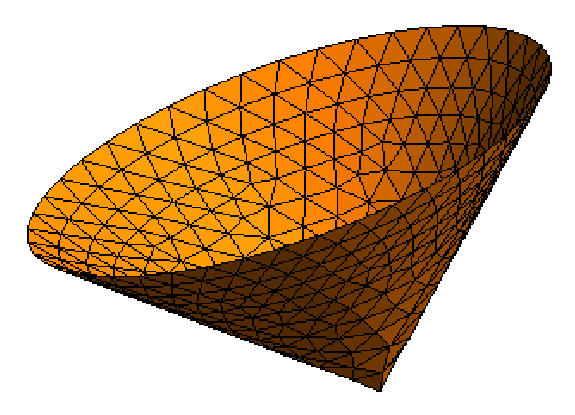
\includegraphics[width=75mm]{cone.eps}}

\verbatim
   Manifold cone_manif = RR3.implicit ( x*x + y*x == z*z );
   cone_manif.implicit ( z == 1. );
   Cell A ( tag::vertex );  x(A) = 1.;  y(A) = 0.;  z(A) = 1.;
   Mesh circle ( tag::progressive, tag::start_at, A,
                 tag::towards, { 0., -1., 0. ),
                 tag::desired_length, 0.1            );
   cone_manif.set_as_working_manifold();
   Cell V ( tag::vertex );  x(V) = 0.;  y(V) = 0.;  z(V) = 0.;
   Mesh cone ( tag::progressive, tag::boundary, circle,
               tag::start_at, A, tag::towards, { -1., 0., -1. },
               tag::singular, V, tag::desired_length, 0.1        );
\endverbatim


\paragraph{\numb section 3.\numb parag 21.
\special{ps: gsave 0.6 setgray}Singularities, again\special{ps: grestore}}

{\bf The code described in this paragraph does not work yet.
It should be regarded as a mere declaration of intentions.}
\medskip

Besides vertices like the one described in paragraph \numb section 3.\numb parag 20, another
kind of singularity appears when we intersect two manifolds which have a tangency point.
This happens if we choose {\codett rc = 0.5} in paragraph \numb section 3.\numb parag 18 or
\numb section 3.\numb parag 19.

We focus on the piece of cylinder from paragraph \numb section 3.\numb parag 19
(which is to be subsequently {\codett join}ed with a sphere with two holes).

\verbatim
   Manifold cylinder = RR3.implicit ( y*y + (z-0.5)*(z-0.5) == 0.25 );
   Manifold infinity = cylinder.implicit ( x*x + y*y + z*z == 1. );
   Cell V ( tag::vertex );  x(V) = 0.;  y(V) = 0.;  z(V) = 1.;
   Mesh circle_1 ( tag::progressive,
                   tag:: start_at, V, tag::towards, { 1., 1., 0. },
                   tag::singular, V, tag::desired_length, 0.1       );
   Mesh circle_2 ( tag::progressive,
                   tag:: start_at, V, tag::towards, { -1., -1., 0. },
                   tag::singular, V, tag::desired_length, 0.1         );

   cylinder.set_as_working_manifold();
   Cell W = circle_1.cell_in_front_of(V).tip();
   Mesh piece_of_cyl ( tag::progressive, tag::boundary, circle_1, circle_2,
                       tag::start_at, W, tag::towards, { -1., 1., 0. },
                       tag::singular, V, tag::desired_length, 0.1           );
\endverbatim

\bigskip
\centerline{\includegraphics[width=85mm]{cyl.eps}}
\bigskip

{\ManiFEM} accepts as {\codett Manifold} a self-intersecting set like {\codett infinity}.
However, in the {\codett Mesh} constructor we must specify {\codett V} as singular point.

Unlike in paragraph \numb section 3.\numb parag 19, here we cannot {\codett join} the two
meshes {\codett circle\_1} and {\codett circle\_2}.
{\ManiFEM} is unable to join two closed polygonal lines having a vertex in common;
in other words, it does not handle self-intersecting {\codett Meshes}.
This is why we provide the two pieces of boundary separately.


\paragraph{\numb section 3.\numb parag 22. Non-uniform meshing}

The {\codett desired\_length} may be a non-constant function.

\verbatim
   Function d = 0.03 + 0.04 * ( (x+0.3)*(x+0.3) + (y-0.9)*(y-0.9) );
   Manifold circle = RR2.implicit ( x*x + y*y == 1. );
   Mesh outer ( tag::progressive, tag::desired_length, d );
   Manifold ellipse = RR2.implicit ( x*x + (y-0.37)*(y-0.37) + 0.3*x*y == 0.25 );
   Mesh inner ( tag::progressive, tag::desired_length, d );
   Mesh bdry ( tag::join, outer, inner.reverse() );
   RR2.set_as_working_manifold();
   Mesh disk ( tag::progressive, tag::boundary, bdry, tag::desired_length, d );
\endverbatim

\centerline{\includegraphics[width=90mm]{disk-non-unif.eps}}
\medskip

Compare with the mesh in paragraph \numb section 3.\numb parag 3.

It is the user's responsibility to provide a {\codett desired\_length} which takes positive
values at all points of the future mesh.
Also, {\codett desired\_length} should be a reasonably smooth function;
sharp variations should be avoided.


\vfil\eject
\paragraph{\numb section 3.\numb parag 23. 
\special{ps: gsave 0.6 setgray}Changing the Riemann metric\special{ps: grestore}}

{\bf The code described in this paragraph does not work yet.
It should be regarded as a mere declaration of intentions.}
\medskip

We can attach a non-uniform metric to our manifold; as a consequence, for a constant
{\codett desired\_length}, the apparent segment length will vary from zone to zone.
For instance, in the code below we set a metric which increases the measured length
of the segments close to the narrow part of the domain.
As a consequence, the meshing algorithm, while trying to build a mesh of constant
{\codett desired\_length}, will choose shorter segments in the proximity of the narrow zone
(because the length measured by the Riemann metric will be larger than the length
we see in the drawing), thus producing the same result as in paragraph
\numb section 3.\numb parag 22.

\verbatim
   Manifold RR2 ( tag::Euclid, tag::of_dim, 2 );
   Function xy = RR2.build_coordinate_system ( tag::Lagrange, tag::of_degree, 1 );
   Function x = xy[0],  y = xy[1];
   Function d = 0.3 + 0.5 * ( (x+0.3)*(x+0.3) + (y-0.9)*(y-0.9) );
   RR2.set_metric ( 1. / d );
   
   Manifold circle = RR2.implicit ( x*x + y*y == 1. );
   Mesh outer ( tag::progressive, tag::desired_length, 0.1 );
   Manifold ellipse = RR2.implicit ( x*x + (y-0.37)*(y-0.37) + 0.3*x*y == 0.25 );
   Mesh inner ( tag::progressive, tag::desired_length, 0.1 );
   Mesh bdry ( tag::join, outer, inner.reverse() );
   RR2.set_as_working_manifold();
   Mesh disk ( tag::progressive, tag::boundary, bdry, tag::desired_length, 0.1 );
\endverbatim

These two approaches (the one described in paragraph \numb section 3.\numb parag 22 and the
one described here) can be used interchangeably.
It is possible to use both in the same code, but the code will become rather obscure.


\paragraph{\numb section 3.\numb parag 24. 
\special{ps: gsave 0.6 setgray}Anisotropic metric\special{ps: grestore}}

{\bf The code described in this paragraph does not work yet.
It should be regarded as a mere declaration of intentions.}
\medskip

The technique described in paragraph \numb section 3.\numb parag 23 can be generalized to
an anisotropic Riemann metric.
We define the metric by means of a square matrix $M$.
$M$ must be symmetric positive definite.
The arguments of {\codett set\_metric} are $ m_{11} $, $ m_{12} $ and $ m_{22} $ for two dimensions,
$ m_{11} $, $ m_{12} $, $ m_{13} $, $ m_{22} $, $ m_{23} $ and $ m_{33} $ for three dimensions.

\verbatim
   Manifold RR2 ( tag::Euclid, tag::of_dim, 2 );
   Function xy = RR2.build_coordinate_system ( tag::Lagrange, tag::of_degree, 1 );
   Function x = xy[0],  y = xy[1];
   Function d = 0.3 + (x+0.3)*(x+0.3) + (y-0.9)*(y-0.9);
   RR2.set_metric ( 1. + 1./d, -3./d, 1. + 9./d );
   // or, equivalently :
   // RR2.set_metric ( tag::principal_part, 1.,
   //                  tag::deviatoric_part, 1./d, -3./d, 9./d );

   Manifold circle = RR2.implicit ( x*x + y*y == 1. );
   Mesh outer ( tag::progressive, tag::desired_length, 0.1 );
   Manifold ellipse = RR2.implicit ( x*x + (y-0.37)*(y-0.37) + 0.3*x*y == 0.25 );
   Mesh inner ( tag::progressive, tag::desired_length, 0.1 );
   Mesh bdry ( tag::join, outer, inner.reverse() );
   RR2.set_as_working_manifold();
   Mesh disk ( tag::progressive, tag::boundary, bdry, tag::desired_length, 0.1 );
\endverbatim

\medskip
\centerline{\includegraphics[width=80mm]{disk-anisotrop.eps}}
\medskip

Compare with the mesh in paragraph \numb section 3.\numb parag 3.

This result cannot be achieved using the approach of paragraph
\numb section 3.\numb parag 22 (by setting a non-constant {\codett desired\_length}).


\paragraph{\numb section 3.\numb parag 25. Future work}

It would be nice to define domains using inequalities between {\codett Function}s.
